%%%%%%%%%%%%%%%%%%%%%%%%%%%%%%%%%%%%%%%%%%%%%%%%%%%%%%%%%%%%%%%%%%%%%%%%%%%%%%%%
%2345678901234567890123456789012345678901234567890123456789012345678901234567890
%        1         2         3         4         5         6         7         8

\documentclass[letterpaper, 10 pt, conference]{ieeeconf}  % Comment this line out if you need a4paper

%\documentclass[a4paper, 10pt, conference]{ieeeconf}      % Use this line for a4 paper

\IEEEoverridecommandlockouts                              % This command is only needed if 
                                                          % you want to use the \thanks command

\overrideIEEEmargins                                      % Needed to meet printer requirements.

%In case you encounter the following error:
%Error 1010 The PDF file may be corrupt (unable to open PDF file) OR
%Error 1000 An error occurred while parsing a contents stream. Unable to analyze the PDF file.
%This is a known problem with pdfLaTeX conversion filter. The file cannot be opened with acrobat reader
%Please use one of the alternatives below to circumvent this error by uncommenting one or the other
%\pdfobjcompresslevel=0
%\pdfminorversion=4

% See the \addtolength command later in the file to balance the column lengths
% on the last page of the document

% The following packages can be found on http:\\www.ctan.org
%\usepackage{graphics} % for pdf, bitmapped graphics files
\usepackage{epsfig} % for postscript graphics files
%\usepackage{mathptmx} % assumes new font selection scheme installed
%\usepackage{times} % assumes new font selection scheme installed
%\usepackage{amsmath} % assumes amsmath package installed
%\usepackage{amssymb}  % assumes amsmath package installed
\usepackage{cleveref}

\title{\LARGE \bf
All We Share is Grid Map: Data-efficient Multi-Robot Exploration System Based Stable Exploring Path
}


% \author{Albert Author$^{1}$ and Bernard D. Researcher$^{2}$% <-this % stops a space
% \thanks{*This work was not supported by any organization}% <-this % stops a space
% \thanks{$^{1}$Albert Author is with Faculty of Electrical Engineering, Mathematics and Computer Science,
%         University of Twente, 7500 AE Enschede, The Netherlands
%         {\tt\small albert.author@papercept.net}}%
% \thanks{$^{2}$Bernard D. Researcheris with the Department of Electrical Engineering, Wright State University,
%         Dayton, OH 45435, USA
%         {\tt\small b.d.researcher@ieee.org}}%
% }


\begin{document}



\maketitle
\thispagestyle{empty}
\pagestyle{empty}


%%%%%%%%%%%%%%%%%%%%%%%%%%%%%%%%%%%%%%%%%%%%%%%%%%%%%%%%%%%%%%%%%%%%%%%%%%%%%%%%
\begin{abstract}
Collaboratively exploring in an unknown environment under limited communication constraints is an essential and challenging task for a multi-robot system.
Robots in a team need to build a shared global map, tell their location within the map, and steer to the unexplored space.
Various Distributed Simultaneous Localization and Mapping (DSLAM) systems offer solutions to localize robots in communication constrained environments, where no external positioning signals and the communication between robots is limited.
However, current DSLAM systems rely on high-precision inter-robot place recognition methods. It is communication-costing to share the complicated feature for inter-robot place recognition and the sensor data for inter-robot relative pose estimation.
In the multi-robot exploration system, each robot's map has already been shared to build a global map.
Thus we use the grid map, instead of the feature and the sensor data, to do inter-robot place recognition and relative pose estimation to reduce data transmission.
Current DSLAM systems are also vulnerable to mistaken place recognition. Thus the robot trajectories need to overlay each other in an area to use the temporal or geometric information to improve the accuracy of place recognition.
However, current multi-robot exploration strategies are usually not stable, which means a big difference between different robots' exploration trajectories for the same space, resulting in a small overlay area.
In this paper, we propose a stable multi-robot exploration method that ensures the consistency of the trajectories when different robots exploring the same area and thus improves the accuracy of place recognition.
\end{abstract}


%%%%%%%%%%%%%%%%%%%%%%%%%%%%%%%%%%%%%%%%%%%%%%%%%%%%%%%%%%%%%%%%%%%%%%%%%%%%%%%%
\section{INTRODUCTION}
Exploring the unknown environment is a basic task for autonomous robot systems.
Multi autonomous robots exploration system can further offer higher time-efficiency, which is especially important for time urgency scenario like rescue after earthquake. Such applications always come with limited facilities where the communication is highly constrainted and even crashes. Thus a multi-robot system for such applications should 1) transmit as less data as possible, and 2) perform exploration either as a single agent without communication or as one of a team when communication is available to faciliate the exploration progress.  
% Jianming: 此处需要给出我们整个系统的核心优势。并且综合论文写 “正确 且 合理” 的场景应用

% Using a team of robots to explore and build the map of an unknown environment is the basic task of many multi-robot applications.
% This work target 2D multi-robot exploration, because current practical applications, such as self-driving cars, home service robots, and multi-robot rescue, are mainly based on 2D AGV platforms.

% Jianming: Based on my understanding, multi-robot rescue will use the height info. then why 2D AGV are listed here?
% Jianming: We'd better not mention 2D/3D for it is one disadvantage of our work. 
% home service robots: 家用机器人为什么要用到多机?
% self-driving cars: 自动驾驶只需要感知,动态路径规划 & 导航,请问为什么哪里需要exploration?

Multi-robot exploration consists of two intertwined stages including perception and decision.
% In terms of perception of multi-robot system, robots in this team need to do Distributed Simultaneous Localization and Mapping (DSLAM) to share their understanding of the environment, build a global map together, and provide the location of each robot in this map.
In the stage of perception, all robots work in the Distributed Simultaneous Localization and Mapping (DSLAM) manner. Specifically, each robot explores its surrounding environment individually. Then robots share their local maps to build a global map together and get their locations in this map.
In the stage of decision, robots navigate themself to explore unknown space, thus expanding the known and explored area of a map.% which is updated while doing the DSLAM.

It is a common practice to use external positioning signals (e.g. GPS, motion capture) to provide the location of the robots. 
Yet in communication constrained environments, such as cave exploration and building inspection, the external positioning signals will be shielded. 
Some previous works implement DSLAM systems \cite{cieslewski2018data, lajoie2020door, schmuck2019ccm} to provide the location in these nonideal environments. 
The basic idea of these DSLAM are similar: 1) adopting single-robot SLAM system to provide intra-robot location, 2) sharing \& matching place recognition infomation to detect the inter-robot loop closures, 3) transmitting the sensor data related to the recognized same place to calculate relative poses (RelPose) and 4) merging \& optimizing the single-robot SLAM results according to the relative poses. 
These systems use camera image to extract a sophisticated feature vector to encode the place information. 
% Computing the distance between feature vectors can know if robots experience the same place. 
These feature vectors can be generated form the handcrafted method \cite{jegou2014triang} or emerging neural-network-based method \cite{radenovic2018fine, arandjelovic2016netvlad}. 
However, these image-based methods are communication-costing for sharing the feature vectors. 
Besides sharing place information, the corresponding sensor data (camera images or laser scans), which are also communication-costing, need to be transmitted between robots to get the relative pose (RelPose).
DSLAM systems are also vulnerable to mistaken place recognition. Some works develop outlier rejection method using temporal information \cite{cieslewski2018data} and geometric verification \cite{lajoie2020door}. 
However, these outlier rejection methods needs the robot trajectories overlap with others in an area to provide extra temporal or geometric constrains.

Frontier-based exploration strategies are usually used in robotic exploration for both single-robot and multi-robot exploration \cite{senarathne2013efficient, umari2017autonomous, orvsulic2019efficient}.
The flow of these frontier-based methods are: 1) detecting points on the frontier edges of the map, which separate the explored space and the unknown space, and 2) assigning one of the frontier point to the robot as its goal for exploration. 
Frontier-based methods can be easily deployed on the real robot with the help of ROS framework \cite{quigley2009ros}, because only one goal point needs to be sent to the robot. 
However, previous works mainly focus on shortening the exploration time and exploring path length. 
When use these methods together with DSLAM systems for multi-robot exploration, the trajectories of different robots may not sufficiently overlap, resulting in the failure of place recognition.

\begin{figure*}[t]
    \centering
    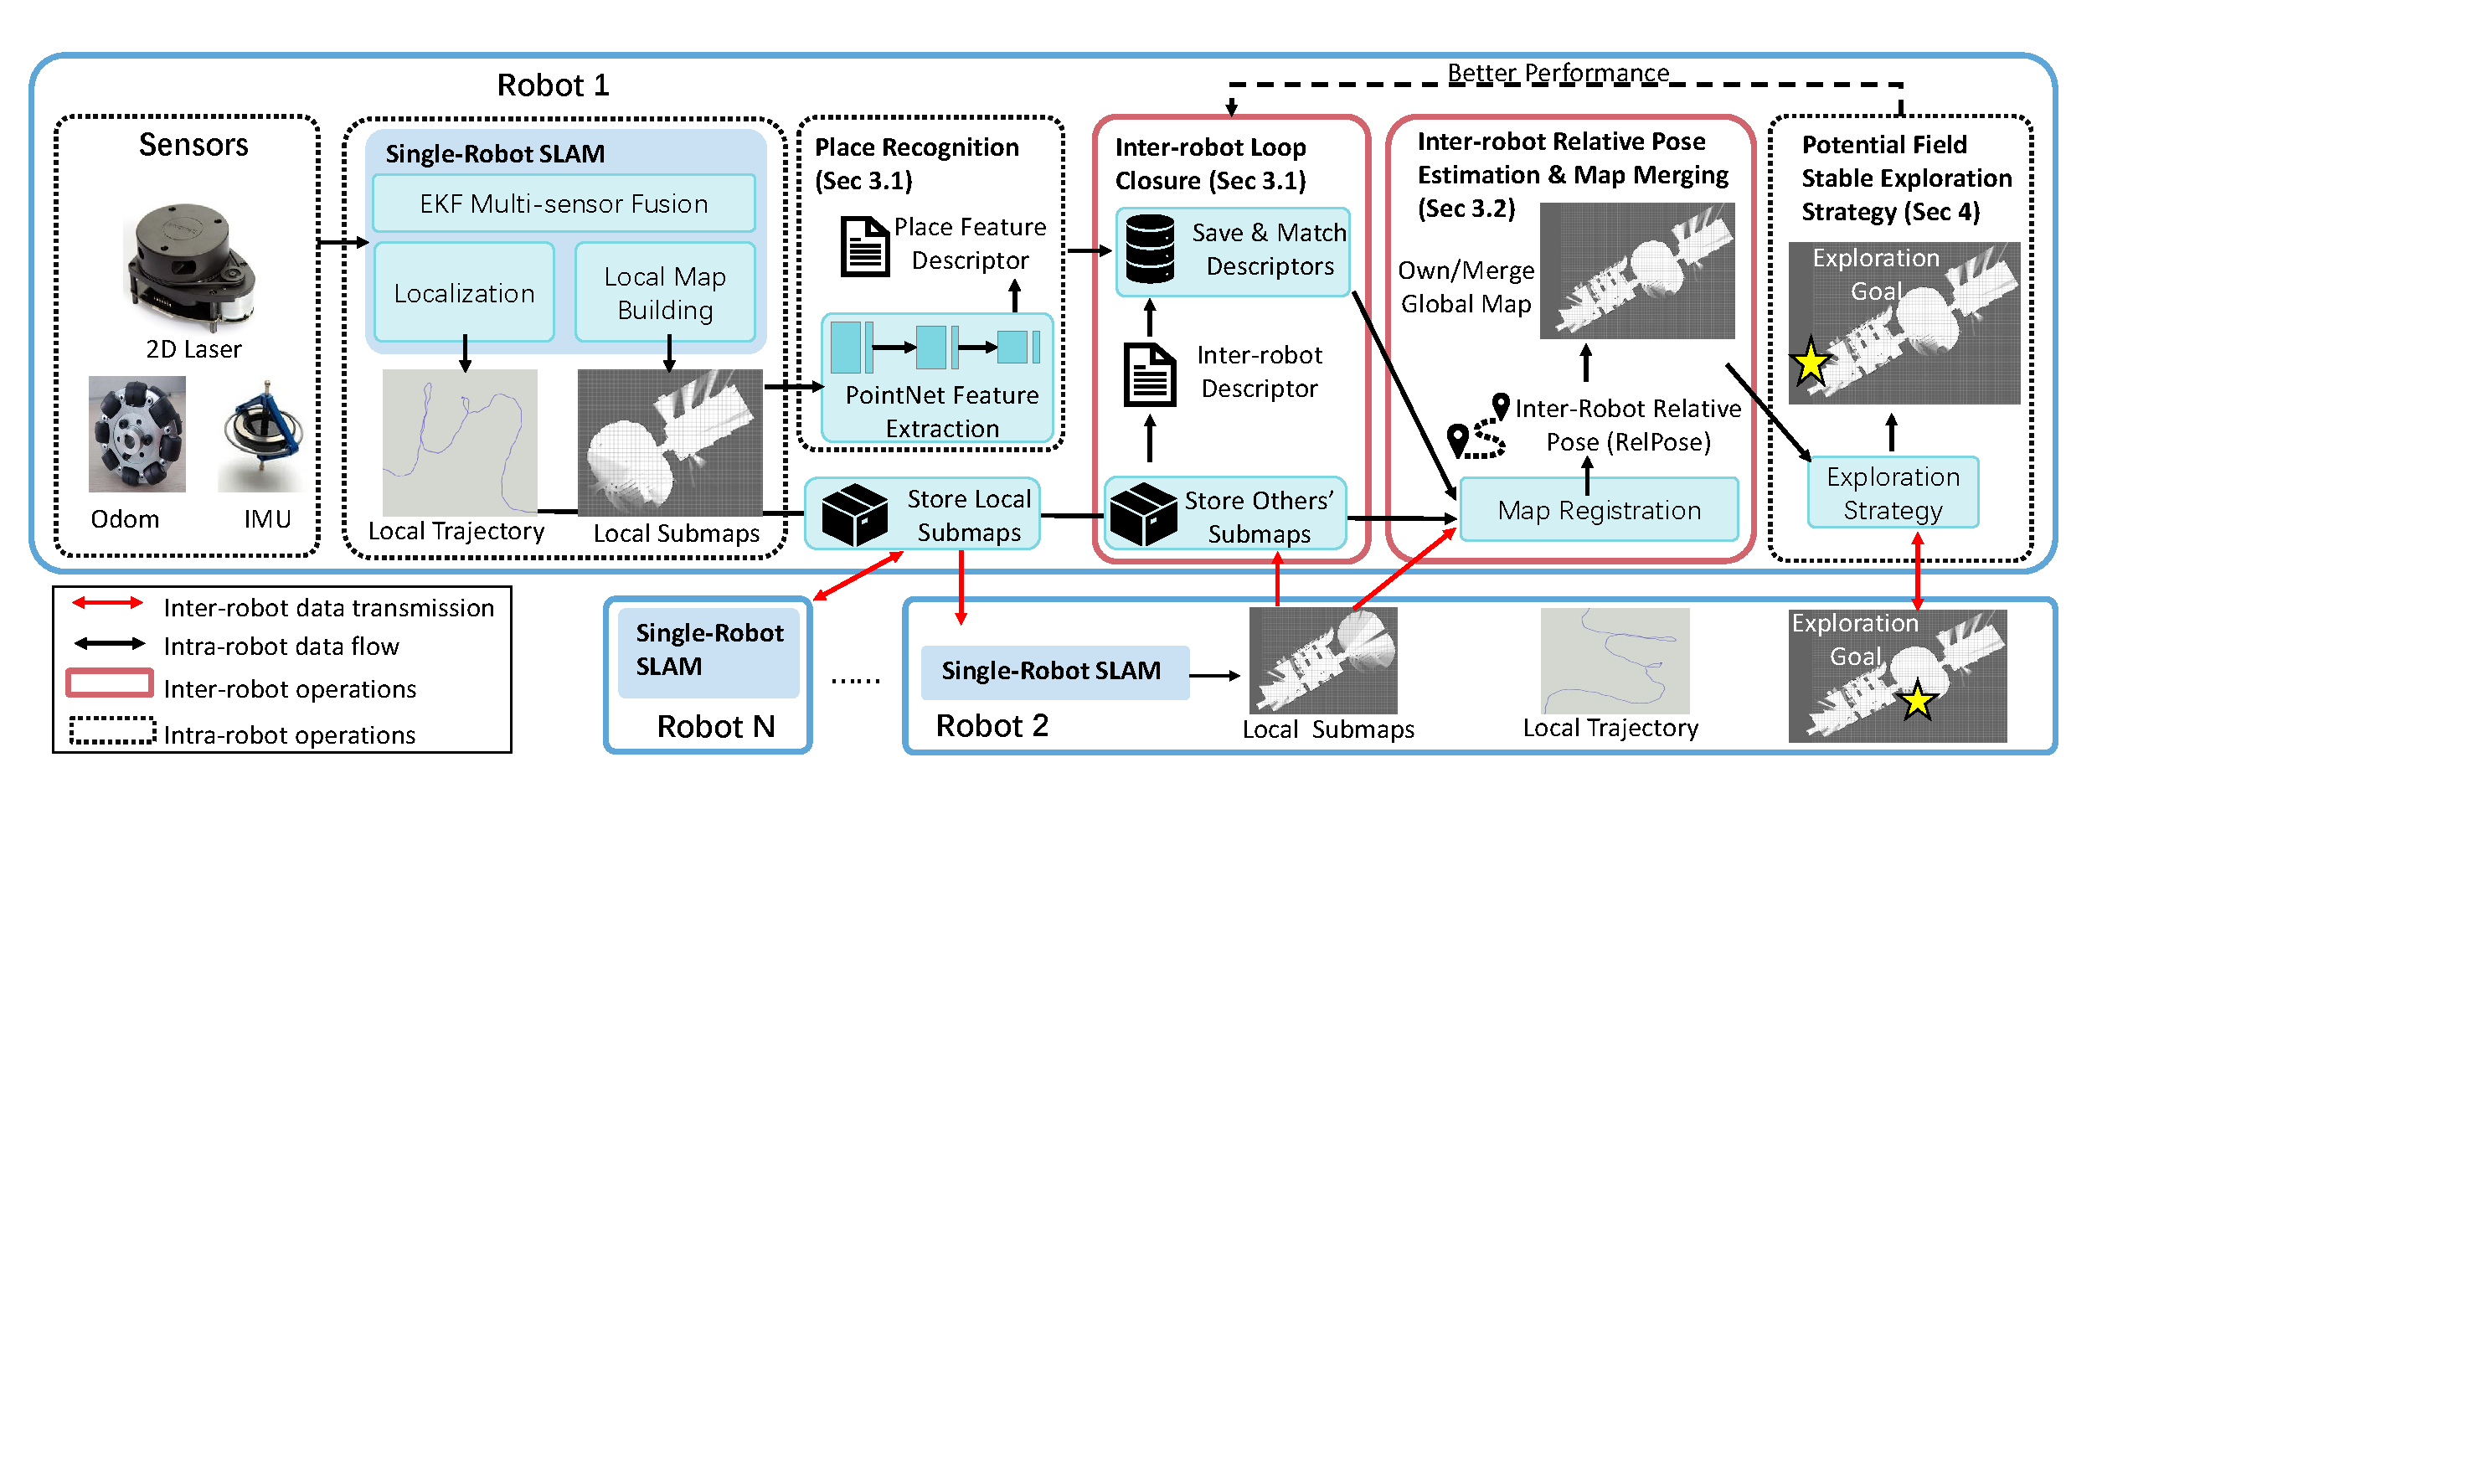
\includegraphics[width=0.99\linewidth]{fig/dataflow.pdf}
    \caption{The system overview of our multi-robot exploration system. All the infomation transmitted between robots are the submaps (the local maps \& the location of each local map on the trajectory). 
    The place descriptor is generated for each self and other's submap. The descriptor is recorded and used for place matching. 
    As the same place are detected between different robots, the relative pose (RelPose) of these robots are also calculated from the shared submaps, and the submaps are merged into a global map. 
    Finally, the stable exploration method will assign each robot to different unknown spaces if they konw the position of each other. 
    Otherwise, the stable exploration method will guide the robots to the explore through a stable path so that they may meet a same place.}
    \label{fig:sysframe}
\end{figure*}

% 多机RRT中心化弊端。

To address the aforementioned problems about communication traffic and place recognition efficiency. We propose a data-efficient multi-robot  exploration system with the following contributions:

\begin{itemize}
    \item A decentralized multi-robot exploration method based on Rapidly Random Tree (RRT) to 
    % \item We use local occupancy grid submaps instead of camera images to extract feature vectors for place recognition. We use neural-network (NN) to provide rich feature for 
    \item A neural network (NN) based map feature extraction method to replace high-precision maps with low-precision maps in place recognition. Thus storage of maps will compressed.
    % For the map description, am I correct?
    \item A map registration method which only feeds on maps without images is proposed to reduce the communication overhead.
    \item Submaps instead of the sensor data are utilized to estimate the relative pose between robots.
    % \item We introduce the idea of potential field to frontier-based exploration strategy to generate stable exploration paths to provide overlapped trajectories for better place recognition performance.
\end{itemize}

As illustrated in \Cref{fig:sysframe}. the single-robot SLAM method (we use Cartographer \cite{hess2016real} in this work) builds the submaps, which include the local map of an area within a region and its location on the exploration trajectory, according to the lidar scan, wheel odometery and IMU sensors.
Each submap is shared between robots, a CNN-based method extracts each submap into a feature vector for further matching to detect inter-robot loop closures.
The submap is also used to estimate the relative pose between robots according to the inter-robot loop closures.
Before detecting the inter-robot loop closures, the robot merge the single-robot local submaps to produce its own global map. 
The stable exploration method will guide the robot on its own global map through a stable path to meet a same place with others while exploring the unknown area.
After detecting the inter-robot loop closures, the robots will merge its own submap and orthers' to build a merged global map. The different robots will be assigned to different unknown area for better exploration efficiency.


The rest of this article is organized as follows: \Cref{sec:relatedwork} introduces the related works. The submap-based DSLAM system is shown in \Cref{sec:dslam}. The stable exploration path generation method is detailed in \Cref{sec:exploration}. The results and evaluation are listed in \Cref{sec:experiment}. \Cref{sec:conclusion} will conclude this paper.

\section{RELATED WORKS}
\label{sec:relatedwork}

\subsection{Inter-robot Loop Closure Detection}
Inter-robot loop closure detection, or place recognition, aligns the trajectories of different robots, based on the sensor frames in the same place. 
It is a common way to generate and compare descriptors to find out the potential loop closure.
For vision-based loop closure detection, there are works to extract feature from input image, such as ORB feature\cite{Mur-Artal:2017281} and SIFT feature \cite{lowe2004distinctive} and use some aggregation method to compact the feature into vectors, such as Bag-of-Word \cite{jegou2011aggregating} and VLAD \cite{tolias2013aggregate}.
Recently, convolutional neural networks (CNN) improve the perfomance of visual place recognition in accuracy and robustnesss, sucn as NetVLAD \cite{arandjelovic2016netvlad} and GeM \cite{radenovic2018fine}.
Different from the rich feature of images, laser scan, especially 2D laser scan, is lack of information. Above image-based algorithms cannot directly applied to the laser sensors, even on the  2D map constructed from laser.
\cite{ribenren1} and \cite{ribenren2} design feature extract method for 2D map. 
However, these method are designed for map registration, yet not applicable for place recognition since the feature is not discriminative.
Recently, some works use neural networks to process laser scan or point cloud, such as PointNet \cite{qi2017pointnet} and PointNetVLAD \cite{angelina2018pointnetvlad}. However, these methods are designed for 3D point clouds and are not suitable for 2D scenes that lack information.
It is still a challenging task to do the place recognition on 2D data, such as 2D scan and 2D map.

\subsection{RelPose Estimation}
Map registration, which is used to calculate the transform (translation and rotation) between two maps belonging to the same place, is the key component of RelPose estimation.
Traditional map registration methods, such as ICP \cite{icp} and NDT \cite{ndt}, use 3D or 2D point clouds as the input and the result of the odometer as the initial transform.
They measure the distance $d$ between the two point clouds $Q_1$ and $Q_2$, adjust the transform to minimize the distance, and then repeat the process until the transform converges.
These methods require a relatively accurate initial transform, otherwise it is easy to converge to a local optimal solution.
For the Single-Robot SLAM, the initial transform can be obtained by the odometer.
But for DSLAM, it is not possible to get the initial transform between different robots.
The mapstitch package \cite{mapstitch} and the map\_merger package \cite{map-merger} use a new map registration method, calculating the transform by the occupancy grids.
They treat the occupancy map as an image, extract and match feature points in different images, and calculate the transform based on the matching result.
This method does not require initial transform and is suitable for DSLAM, but the registration accuracy is lower than traditional methods.

\subsection{Space Exploration Strategy}


\section{SUBMAP-BASED DSLAM}
\label{sec:dslam}
As illustraded in \Cref{fig:sysframe} there are tow main inter-robot components in DSLAM system: 1) place recognition and matching. 2) inter-robot relative pose (RelPose) estimation. In this section we implement these components both based on submaps.

\subsection{Submap-Based Place Recognition}
The key problem of place recognition is to extrct discriminative feature vector from 2D submap.

\subsection{Submap-Based RelPose Estimation}
% Because submap contains the position of the map at the single-robot trajectory, the RelPose of two robots can be estimated by calculating the pose of two submaps in the same scene, which is well defined as map registration.

\begin{figure}[t]
    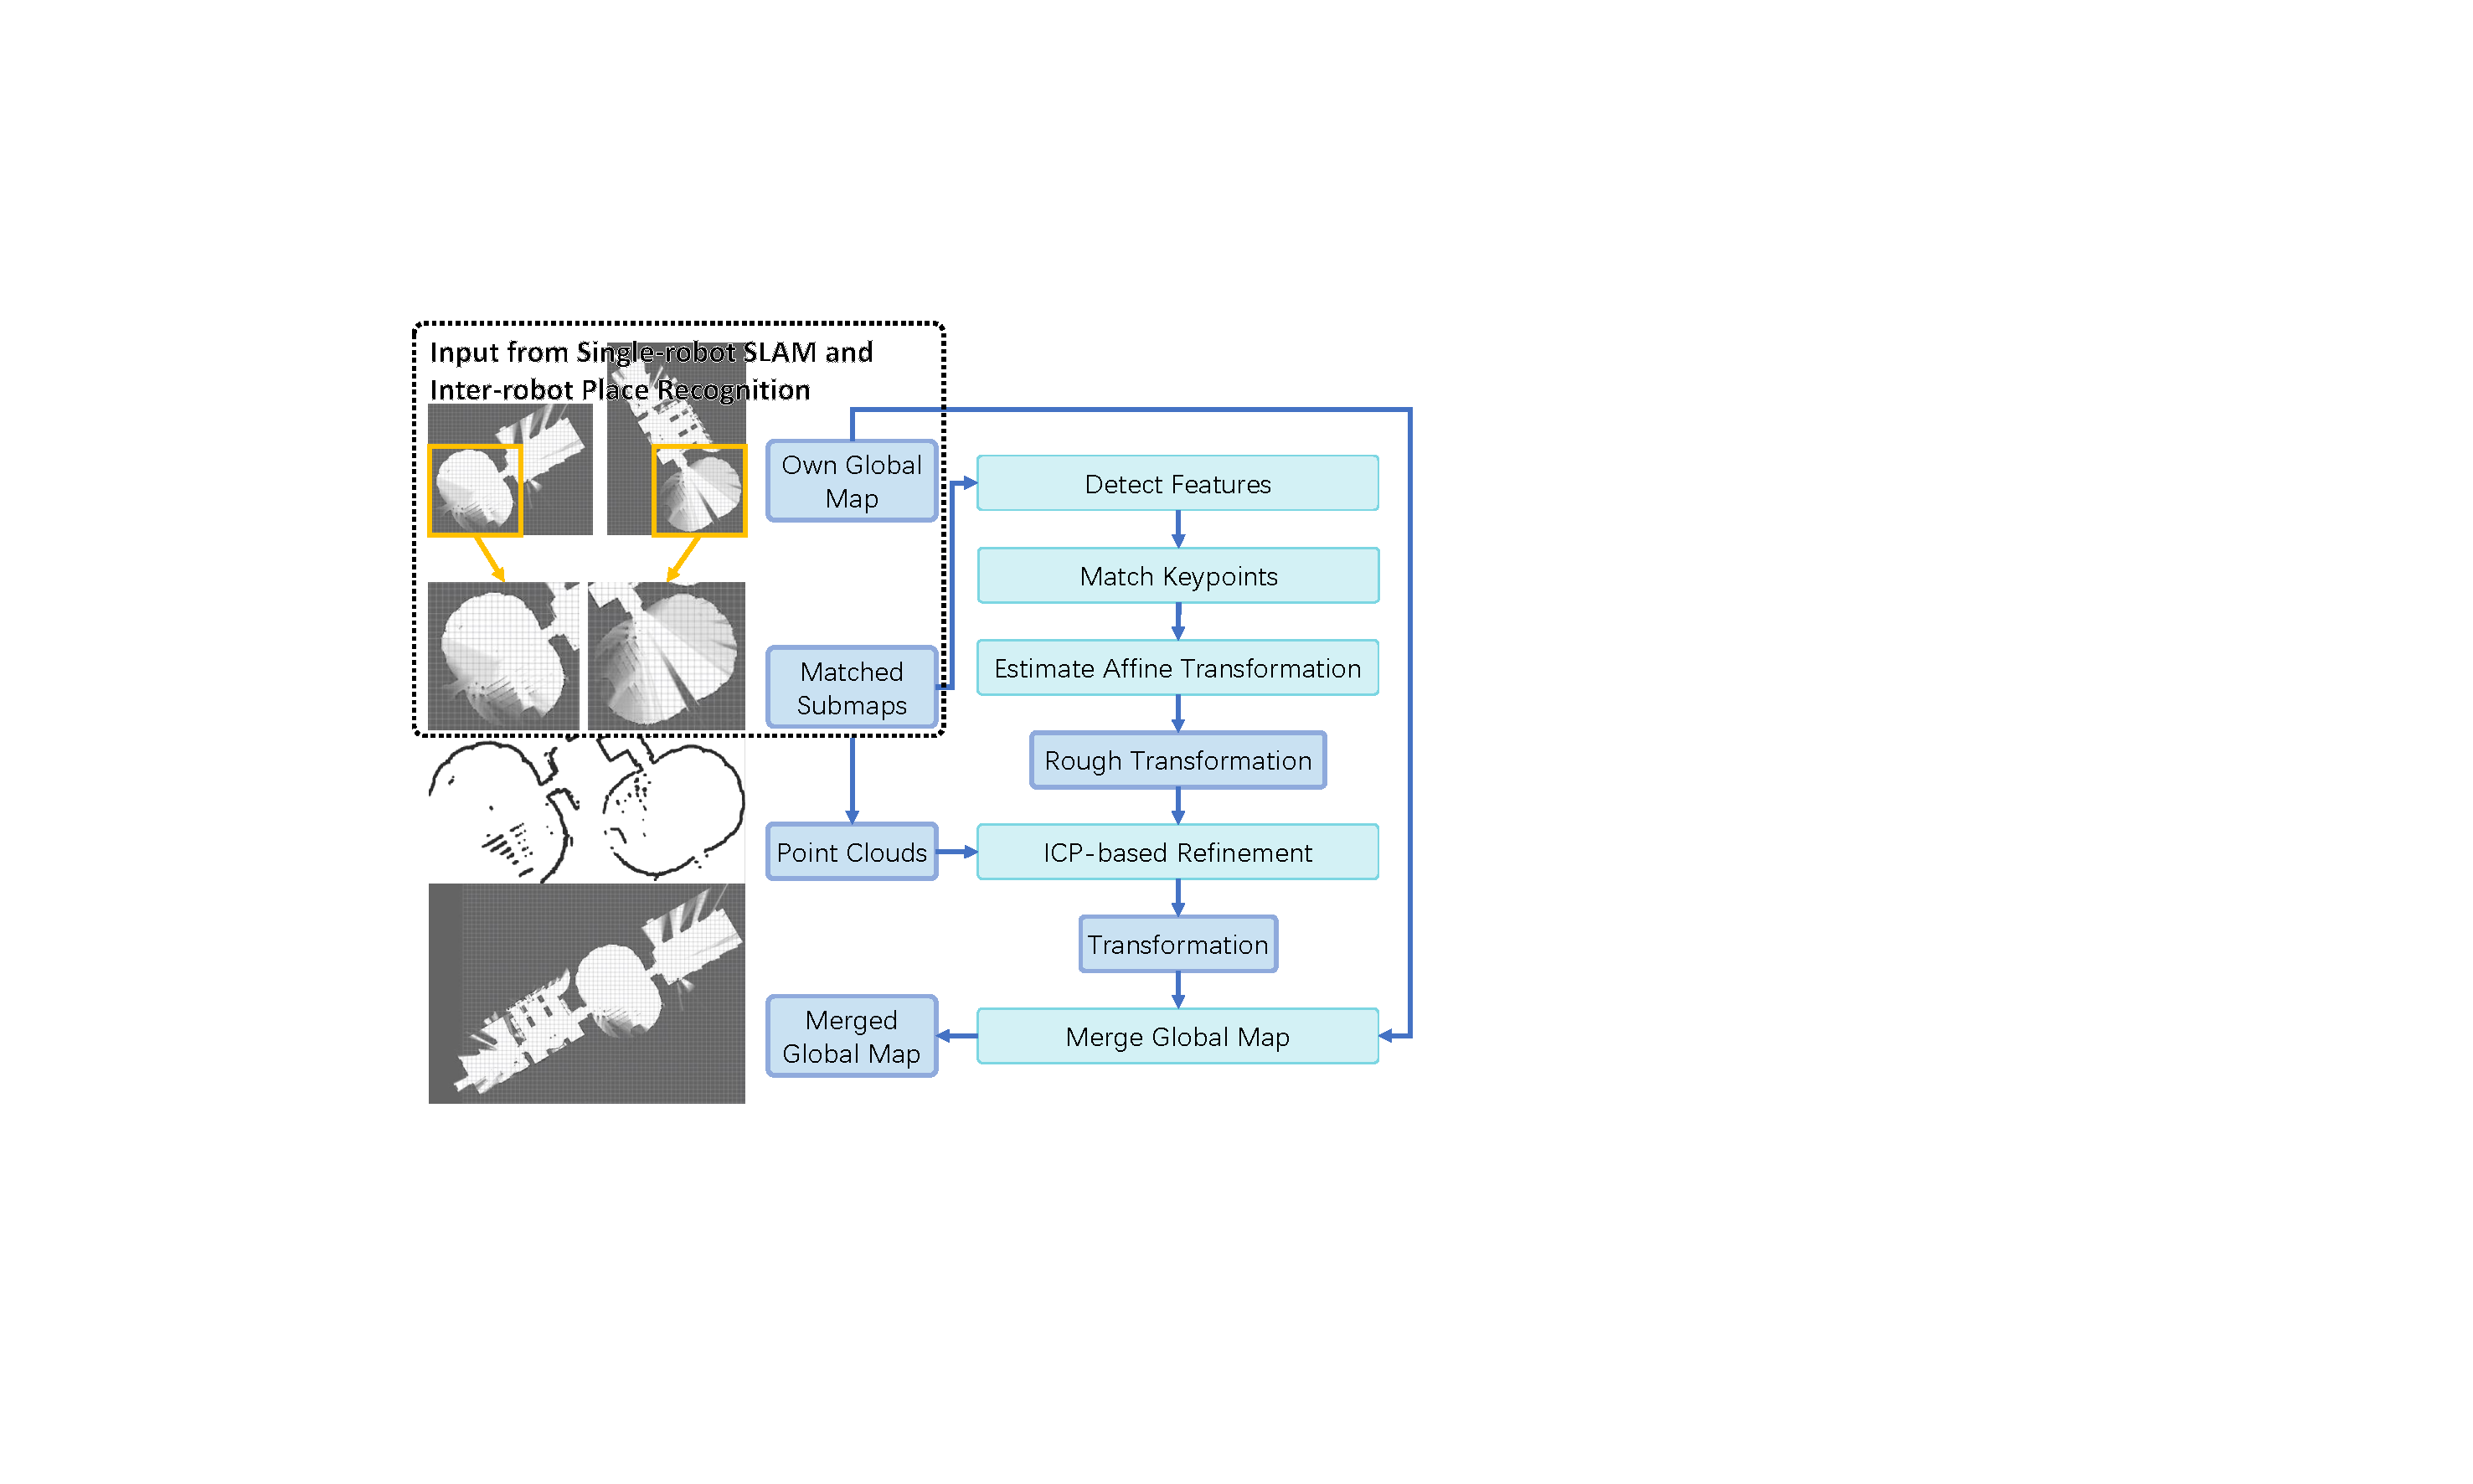
\includegraphics[width=0.99\linewidth]{fig/registration.pdf}
    \caption{An overview of the proposed method for relative pose estimation and map merging.}
    \label{fig:registration}
\end{figure}

We extract image-based features from submap and perform coarse registration. 
After that, we convert the submap to the point cloud and refine the registration result.
Firstly, we extract image-based features like AKAZE, ORB, SURF, etc.
We use the features matcher which finds two best matches for each feature and leaves the best one only if the ratio between descriptor distances is greater than the threshold.
And we check the geometric consistency of the matching results and delete incorrect matches.
After that, the inter-robot transformation can be estimated as the initial value of ICP.
Submaps are converted into point clouds for the refinement of the registration result based on ICP.
The map merger merges the own global maps according to the registration results to obtain the merged global map.

\section{STABLE EXPLORATION}
\label{sec:exploration}

\section{EXPERIMENT RESULT}
\label{sec:experiment}

\section{CONCLUSION}
\label{sec:conclusion}

\bibliographystyle{IEEEtran}
\bibliography{src/fpgaslam}

\end{document}
